\documentclass{article}
\usepackage{graphicx}
\usepackage[utf8]{inputenc}
\usepackage[english]{babel}
\usepackage{amsmath}
\usepackage{hyperref}
\usepackage{amsthm}
\usepackage{tcolorbox}
\usepackage{amsfonts}
\usepackage{amssymb}
\usepackage{mathrsfs}
\usepackage{centernot}
\usepackage{cases}
\usepackage{physics}
\usepackage[shortlabels]{enumitem}
\usepackage{tikz}
\usepackage{lipsum}
\usepackage{sidecap}
\usepackage{verbatim}
\usepackage{listings}
\usepackage{float}

\definecolor{borderblue}{HTML}{33c2ff}
\definecolor{codegreen}{rgb}{0,0.6,0}
\definecolor{codegray}{rgb}{0.5,0.5,0.5}
\definecolor{codepurple}{rgb}{0.58,0,0.82}
\definecolor{backcolour}{rgb}{0.95,0.95,0.92}

\lstdefinestyle{mystyle}{
    backgroundcolor=\color{backcolour},
    commentstyle=\color{codegreen},
    keywordstyle=\color{magenta},
    numberstyle=\tiny\color{codegray},
    stringstyle=\color{codepurple},
    basicstyle=\ttfamily\footnotesize,
    breakatwhitespace=false,
    breaklines=true,
    captionpos=b,
    keepspaces=true,
    numbers=left,
    numbersep=5pt,
    showspaces=false,
    showstringspaces=false,
    showtabs=false,
    tabsize=2
}

\lstset{style=mystyle}

\newcommand{\paren}[1]{\left(#1\right)}
\newcommand{\curly}[1]{\left\{#1\right\}}

\allowdisplaybreaks

\makeatletter
\long\def\paragraph{%
  \@startsection{paragraph}{4}%
  {\z@}{2ex \@plus 1ex \@minus .2ex}{-1em}%
  {\normalfont\normalsize\bfseries}%
}
\makeatother

\makeatletter
\def\@xequals@fill{\arrowfill@\Relbar\Relbar\Relbar}
\newcommand*\xequals[2][]{\DOTSB\ext@arrow0055\@xequals@fill{#1}{#2}}
\makeatother

\makeatletter
\renewcommand*\env@matrix[1][*\c@MaxMatrixCols c]{%
  \hskip -\arraycolsep
  \let\@ifnextchar\new@ifnextchar
  \array{#1}}
\makeatother

\NewTColorBox{algorithm}{m}{
  standard jigsaw,
  sharp corners,
  boxrule=0.4pt,
  coltitle=black,
  colframe=black,
  opacityback=0,
  opacitybacktitle=0,
  fonttitle=\normalfont\bfseries\upshape,
  fontupper=\normalfont,
  title={Algorithm #1},
  after title={.},
  attach title to upper={\ },
}

\title{\textbf{\Huge CulTour }\\
AI-powered Smart Tourism Application}
\author{\textbf{Group 5: deptrAI}}

\date{\today}

\begin{document}

\maketitle

\pagebreak
\tableofcontents
\pagebreak

\section{Team Information}
\lipsum[1]
\section{Idea}

The core concept of \textbf{CulTour} is to re-engineer how cultural tourism is consumed by shifting the paradigm from \textit{Location-Based Services} to a \textbf{Semantic and Visual Discovery Engine}.

While the global travel industry is shifting towards experiential travel, digital tools have remained stagnant. Current platforms treat cultural sites as static geographical points, ignoring the rich historical and sociological context that defines them. CulTour decouples "culture" from mere location, breaking it down into granular, queryable data points such as \textit{Architecture Style}, \textit{Dynastic Era}, \textit{Religious Affiliation}, and \textit{Social Function}.

By treating cultural attributes as structured data rather than unstructured text, CulTour aims to solve the ``Staged Authenticity'' problem. It empowers users to bypass the curated ``front-stage'' of mass tourism and algorithmically locate the ``back-stage'' reality of Vietnamese daily life using a \textbf{Utility-First} approach.

\subsection{Problem Statement}

The tourism sector in Vietnam suffers from a dual failure: a sociological failure of authenticity and a technical failure of information categorization.

\subsubsection{The Sociological Problem}
Cultural tourism often presents a sanitized, curated performance designed to meet perceived tourist expectations. This creates a ``front-stage'' reality where visitors interact with a manufactured version of Vietnam, while the ``back-stage''—the authentic, unstaged aspects of local life—remains hidden.
\begin{itemize}
  \item \textbf{The Gap:} Guided tours (e.g., ``We Show You Saigon!'') focus exclusively on high-traffic, commercialized zones.
  \item \textbf{The Demand:} There is a massive market friction; 77\% of travelers explicitly seek authentic experiences\footnote{\href{https://news.booking.com/bookingcoms-2025-research-reveals-growing-traveler-awareness-of-tourism-impact-on-communities-both-at-home-and-abroad/}{Booking.com 2025 Travel Predictions}} \footnote{\href{https://stories.hilton.com/2025trends/slow-travel-the-growing-desire-to-travel-like-a-local}{Hilton 2025 Slow Travel}}, yet the market primarily supplies generic sightseeing.
\end{itemize}

\subsubsection{The Technical Problem}
The primary barrier to finding authentic experiences is not a lack of existence, but a lack of \textit{discoverability}. Market leaders like Google Maps, Agoda, and Traveloka are optimized for logistics and commerce, leading to a ``flattening'' of cultural value.

\begin{enumerate}
  \item \textbf{The ``Pagoda Problem'' (Taxonomic Failure):} To a standard map algorithm, a 19th-century pagoda with rare Sino-Vietnamese architecture is categorized identically to a newly built concrete pagoda. The platforms lack the semantic depth to distinguish \textit{historical significance} from \textit{utility}.
  \item \textbf{Algorithmic Bias via Popularity:} Recommendation engines on current platforms prioritize venues with high traffic and English reviews. This creates a feedback loop that continually pushes tourists toward ``tourist traps,'' burying authentic, quieter locations under a layer of noise.
\end{enumerate}

\subsubsection{The Information Asymmetry}
Foreign travelers face a ``knowledge wall''.
\begin{itemize}
  \item \textbf{Local Sources:} High-quality blogs analyzing deep culture are predominantly written in Vietnamese, often verbose, and lack structured metadata.
  \item \textbf{English Sources:} Available English resources are often superficial, repetitive, and lack the specific domain knowledge required to explain \textit{why} a location is culturally significant.
\end{itemize}

\subsection{Target Users}

We define our users not just by demographics, but by their search behavior and intent

\subsubsection{The Authenticity Seeker}
Independent travelers or expatriates who want to understand the \textit{context} of what they are seeing. They are unsatisfied by the generic nature of Google Maps categories and are looking for a tool that filters for specific cultural nuance (e.g., ``Find me a temple that is currently active, not just a museum'').

\subsubsection{The Culturally Overwhelmed}
This user wants to engage with local culture but lacks the time or research skills to parse through hundreds of Vietnamese blogs. They find the current volume of unstructured information overwhelming and require a curated, trusted filter to guide them to high-value experiences.

\subsection{System Objectives}

To bridge the gap between foreign curiosity and local reality, the system has four distinct objectives:

\begin{itemize}
  \item \textbf{Construct a Cultural Knowledge Graph}: the system must move beyond keyword matching. It aims to build a semantic engine that understands the relationships between cultural entities.
  \item \textbf{Granular, Attribute-based Search}: the system must solve the ``Pagoda Problem'' by allowing users to filter based on deep attributes rather than surface-level categories.
  \item \textbf{Automated Curation via Preference Matching}: to address the ``overwhelmed'' user, the system will utilize user constraints to auto-curate itineraries.
  \item \textbf{The ``Utility-First'' Adoption Strategy}: we assume that organizers of authentic local events are difficult to onboard immediately.
\end{itemize}
\section{System Overview}
\subsection{Core Functions}
\subsubsection{Granular Search Service}

The search pipeline is built upon a hybrid architecture that combines semantic search and lexical search techniques to optimize both relevance and precision in results. The key components of this pipeline are as follows:

% Changed [htbp] to [H] to force exact placement
\begin{figure}[H]
  \centering
  \includegraphics[width=1.0\linewidth]{externals/uml/ImageSearchPipeline.png}
\end{figure}

% As detailed in Figure \ref{fig:image_pipeline}, the visual search subsystem (Heritage Fusion) operates in three distinct phases:
% \begin{enumerate}
%     \item \textbf{Offline Training:} Public datasets (WikiArt, AHE) are utilized to fine-tune a CLIP ViT-B-16 model via contrastive loss training to better grasp artistic context.
%     \item \textbf{Ingestion Pipeline:} A sequential, memory-optimized GPU process extracts features using a frozen DINOv2 encoder (for style) and the fine-tuned CLIP model (for meaning), while RAM++ generates text tags.
%     \item \textbf{Online Retrieval:} User queries utilize a hybrid fusion approach within a Qdrant Vector DB, calculating a weighted sum of Style and Meaning scores to retrieve and rank the top 5 most relevant results.
% \end{enumerate}

% Changed [htbp] to [H] to force exact placement
\begin{figure}[H]
  \centering
  \includegraphics[width=0.8\linewidth]{externals/uml/GranularSearchPipeline.png}
\end{figure}

\subsubsection{Community Event Service}
This module functions as a dynamic bridge between local culture providers and users, fostering active participation rather than passive observation.

\begin{itemize}
    \item \textbf{Passive Discovery Engine:} The system automatically surfaces active festivals and events by correlating temporal data with location-specific tags. For example, a user browsing a specific pagoda will be notified of upcoming religious rites relevant to that location's history.
    \item \textbf{Decentralized Event Hosting:} Cultural organizations and community leaders are provided with a "Self-hosting" portal. This allows them to create, manage, and broadcast community-driven events directly to interested users, bypassing traditional media gatekeepers.
    \item \textbf{Cultural Differentiation:} Unlike standard event aggregators, this service focuses exclusively on participatory cultural activities, distinguishing the platform as a hub for deep community engagement rather than general entertainment.
\end{itemize}
\subsubsection{Community Event Service}
This module functions as a dynamic bridge between local culture providers and users, fostering active participation rather than passive observation.

\begin{itemize}
    \item \textbf{Passive Discovery Engine:} The system automatically surfaces active festivals and events by correlating temporal data with location-specific tags. For example, a user browsing a specific pagoda will be notified of upcoming religious rites relevant to that location's history.
    \item \textbf{Decentralized Event Hosting:} Cultural organizations and community leaders are provided with a "Self-hosting" portal. This allows them to create, manage, and broadcast community-driven events directly to interested users, bypassing traditional media gatekeepers.
    \item \textbf{Cultural Differentiation:} Unlike standard event aggregators, this service focuses exclusively on participatory cultural activities, distinguishing the platform as a hub for deep community engagement rather than general entertainment.
\end{itemize}

\subsubsection{Recommendation System}
The recommendation engine employs a hybrid filtering approach to personalize the user experience, transforming raw interaction data into curated cultural journeys.

\begin{itemize}
    \item \textbf{Explicit \& Implicit Feedback Loops:} The system captures explicit signals (likes, dislikes) and implicit behaviors (visit history, dwell time, view counts). These inputs are used to build a dynamic user preference profile.
    \item \textbf{Preference Clustering:} By analyzing frequently selected tags (e.g., "Gothic Architecture," "Cham Culture") and visited locations, the algorithm identifies user cohorts with similar tastes. This allows for collaborative filtering, where a user is recommended niche locations that were highly rated by others in their "taste cluster," facilitating serendipitous discovery of new cultural sites.
\end{itemize}
\subsection{Innovation Highlights}
\textbf{Unified Multimodal Search Interface:} Unlike traditional travel platforms restricted to rigid keyword inputs, our system enables a seamless search-by-anything experience. Users can discover locations using natural language prompts, visual inputs, categorical filters, or direct entity names. This flexibility bridges the gap between vague user intent and specific cultural data.

% --- Example Table ---
\begin{table}[htbp]
\centering
\caption{Examples of Multimodal Search Capabilities}
\label{tab:query_examples}
\renewcommand{\arraystretch}{1.3} % Adds padding to rows
\begin{tabular}{|p{3.5cm}|p{10cm}|}
\hline
\textbf{Search Modality} & \textbf{Example User Inputs} \\
\hline
\textbf{Natural Language} & "Quiet places in Saigon to read a book with colonial architecture" \newline "Where can I see traditional water puppet shows?" \\
\hline
\textbf{Visual Input} & \textit{[User uploads photo of Notre Dame Cathedral]} $\rightarrow$ System finds similar Gothic/Romanesque churches. \\
\hline
\textbf{Categorical Filters} & \texttt{\{ "arch\_style": "French Colonial", "district": "1" \}} \newline \texttt{\{ "religion": "Buddhism", "active\_worship": true \}} \\
\hline
\textbf{Direct Entity Lookup} & "Ben Thanh Market" \newline "Ho Chi Minh City Fine Arts Museum" \\
\hline
\end{tabular}
\end{table}

\section{Sequence Diagram}

\subsection{Sign in}
\begin{figure}[H]
    \centering
    \includegraphics[width=\textwidth]{sequence_diagrams/Sign_in.png}
    \caption{Sign in sequence diagram}
    \label{fig:sign_in}
\end{figure}

\subsection{Sign up}
\begin{figure}[H]
    \centering
    \includegraphics[width=\textwidth]{sequence_diagrams/Sign_up.png}
    \caption{Sign up sequence diagram}
    \label{fig:sign_up}
\end{figure}

\subsection{Create Event}
\begin{figure}[H]
    \centering
    \includegraphics[width=\textwidth]{sequence_diagrams/Create_event.png}
    \caption{Create event sequence diagram}
    \label{fig:create_event}
\end{figure}

\subsection{Subscribe Event}
\begin{figure}[H]
    \centering
    \includegraphics[width=\textwidth]{sequence_diagrams/Subscribe_event.png}
    \caption{Subscribe event sequence diagram}
    \label{fig:subscribe_event}
\end{figure}

\subsection{Search Places}
\begin{figure}[H]
    \centering
    \includegraphics[width=\textwidth]{sequence_diagrams/Search_places.png}
    \caption{Search places sequence diagram}
    \label{fig:search_places}
\end{figure}

\subsection{Save Location}
\begin{figure}[H]
    \centering
    \includegraphics[width=\textwidth]{sequence_diagrams/Save_location.png}
    \caption{Save location sequence diagram}
    \label{fig:save_location}
\end{figure}

\subsection{Map Feature}
\begin{figure}[H]
    \centering
    \includegraphics[width=\textwidth]{sequence_diagrams/Map_feature.png}
    \caption{Map feature sequence diagram}
    \label{fig:map_feature}
\end{figure}

\section{Class Diagram}
\subsection{Architecture Overview}
Our system's architecture employs a foursome design pattern, dividing the application into four main layers: the AI backend, the backend, the database, and the frontend. Each layer has distinct responsibilities and interacts with other layers to ensure seamless functionality.

\newpage 

\subsection{Class Diagrams}
\subsubsection{Overall Architecture}
\begin{figure}[h]
  \centering
  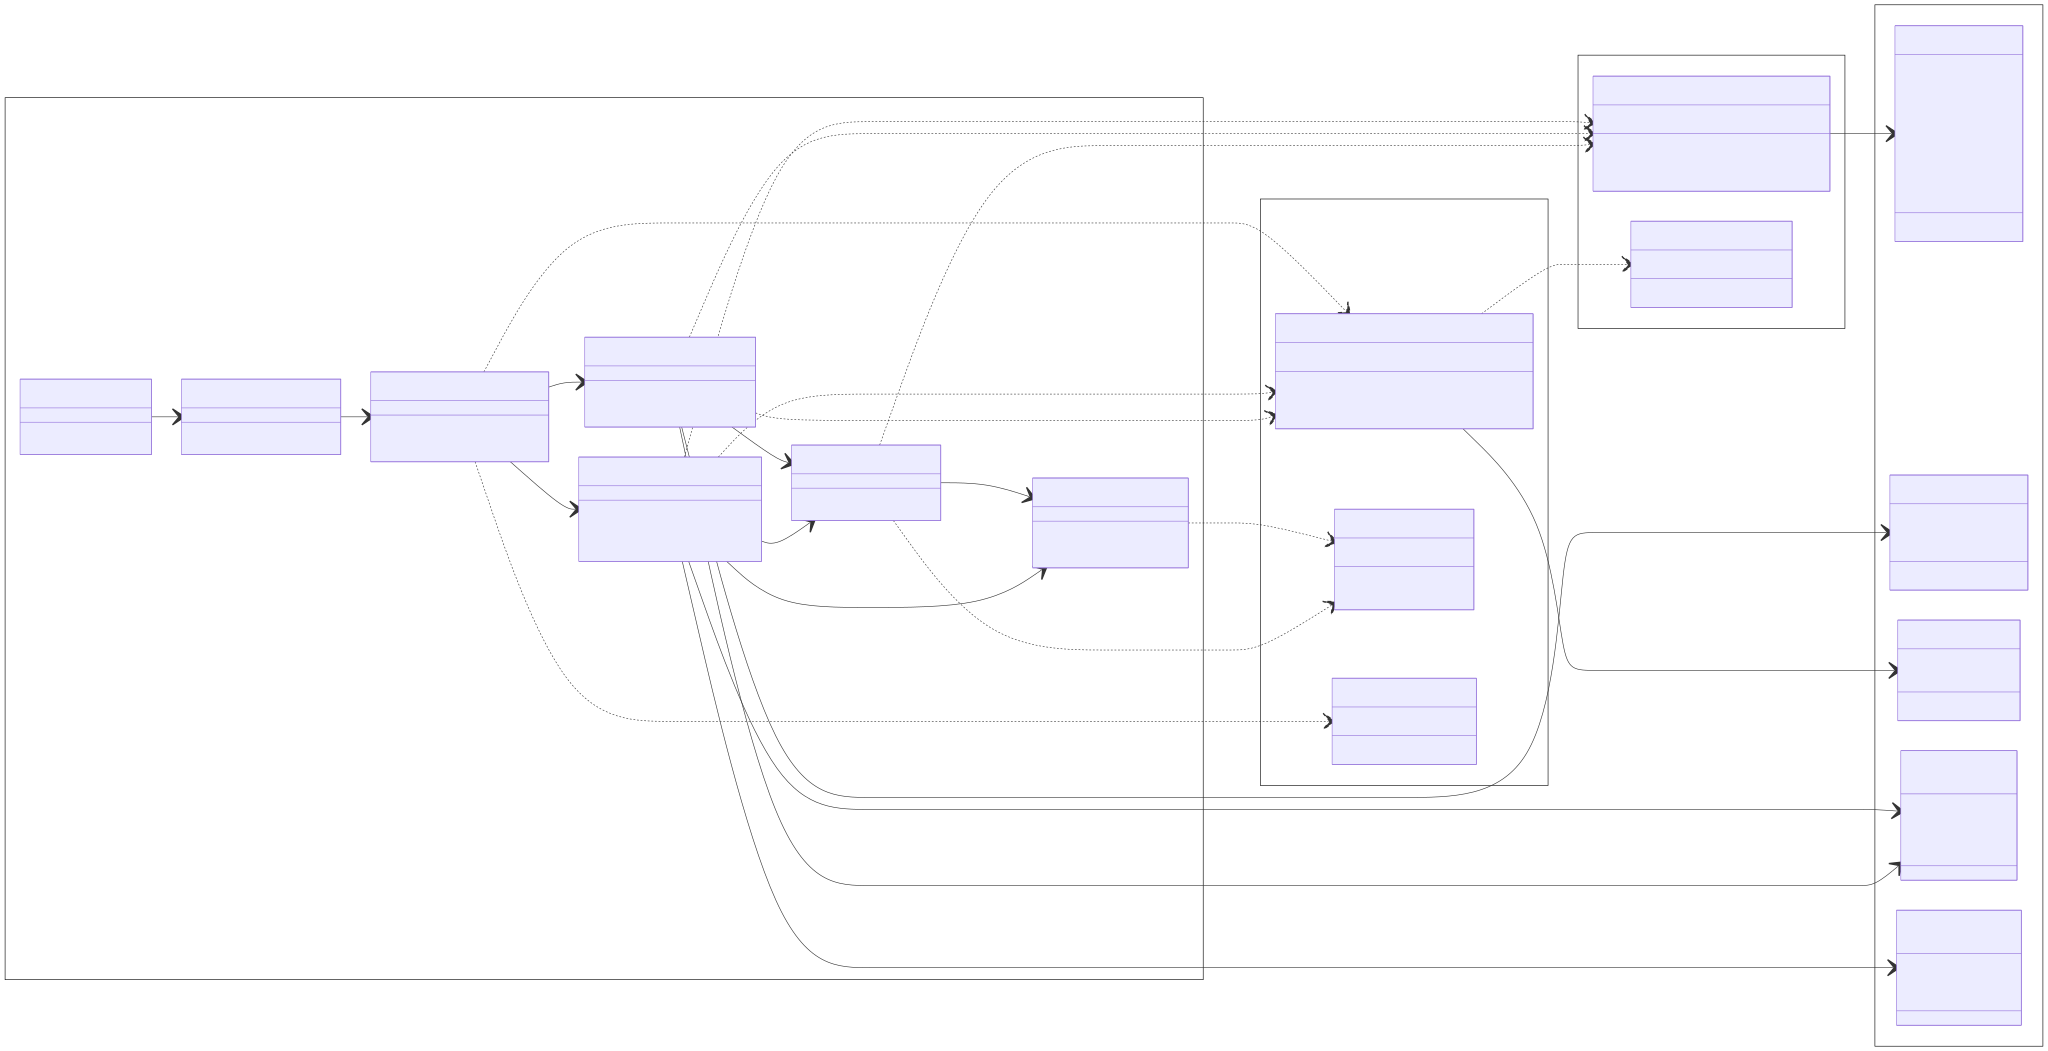
\includegraphics[width=\linewidth]{uml/class-diagram.svg}
  \caption{Overall architecture.}
\end{figure}

\quad The class diagram above illustrates the overall architecture of the system. It shows a Flutter frontend with UI screens (MyApp, IntroductionScreen, HomeScreen, SearchScreen, RegionOverview, PlaceOverview, MapScreen) connected by navigation edges. State is managed via Riverpod providers: UserSessionProvider (user state and preferences), SelectedPlaceProvider (current place), and NavigationIndexProvider (current tab). Service layer classes (PlaceService, ProfileService) wrap Dio HTTP calls to fetch places (by query, ID, or image) and user profiles. Models include Place, Region, User, and enum types FilterType and CategoryType. Screens read or set provider state: Home/Search/Region read UserSession; PlaceOverview sets SelectedPlace; MapScreen listens to SelectedPlace; Home sets NavigationIndex. Services supply data to UI and providers, and models represent the domain entities and filters used across the app.
\newpage

\subsubsection{AI Backend, Backend, and Database}                                                                                                                                                       
\begin{figure}[h]
  \centering
  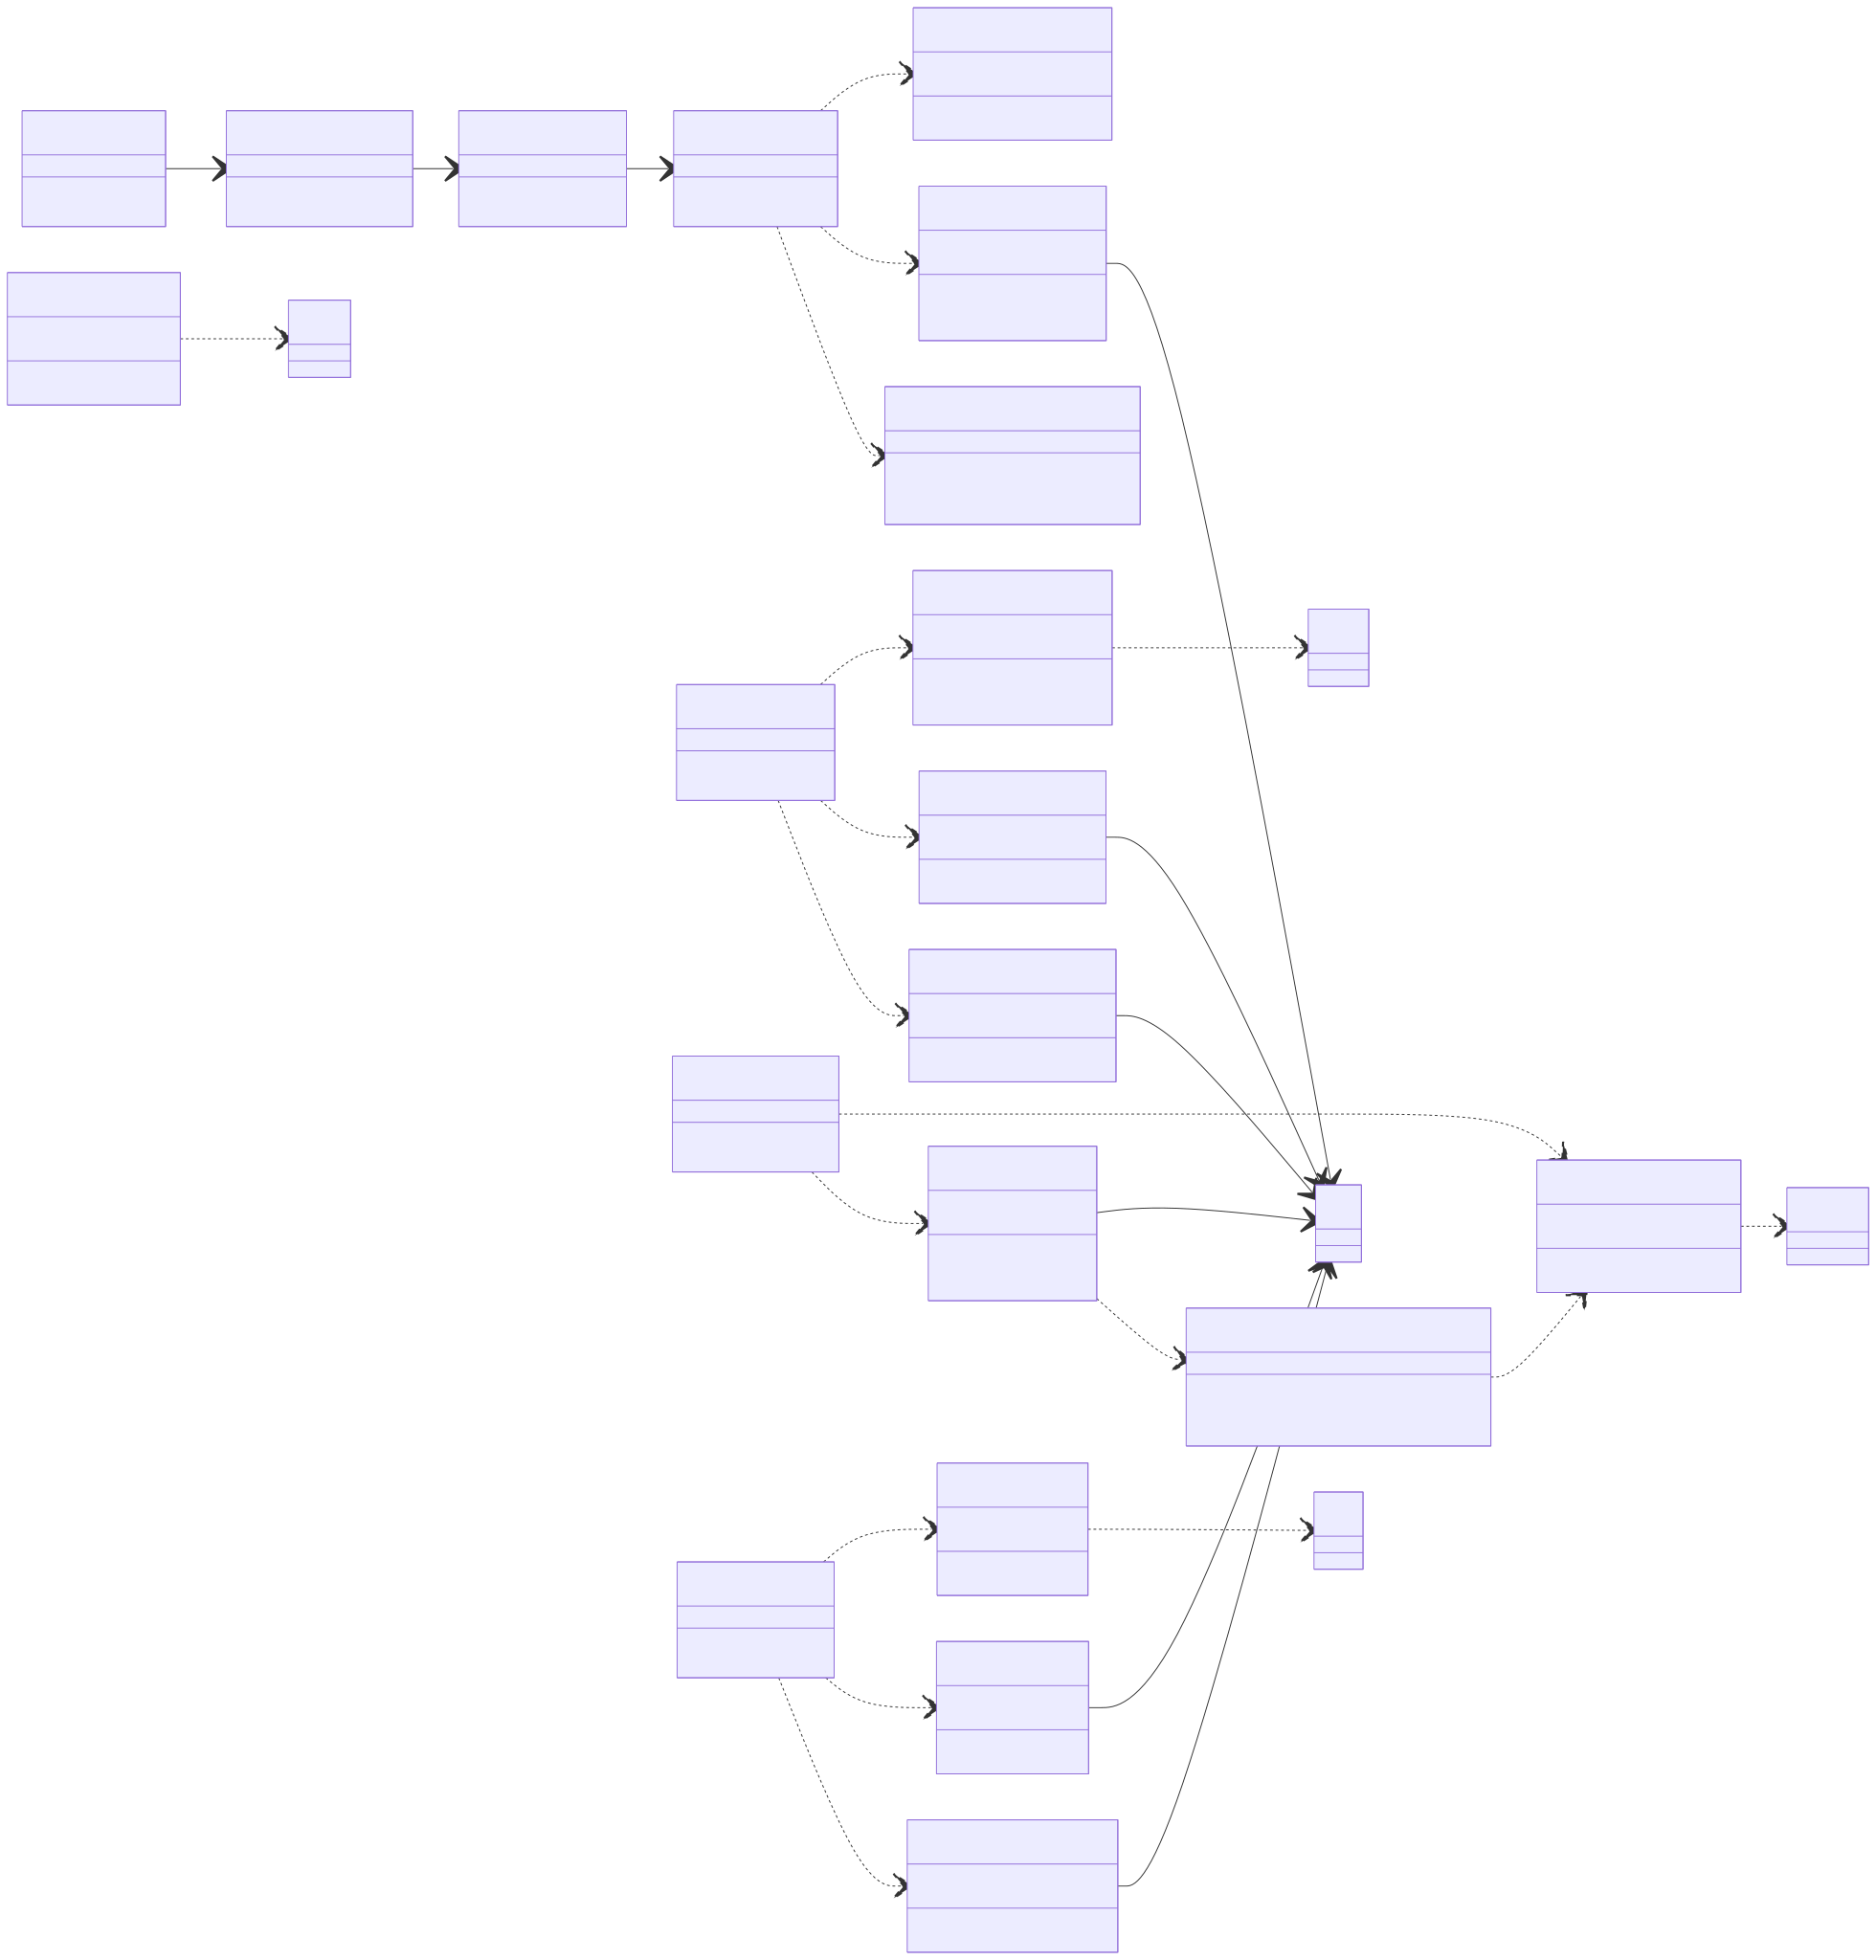
\includegraphics[width=\linewidth]{uml/class-diagram-frontend.svg}
  \caption{Frontend architecture.}
\end{figure}

\quad The Flutter frontend boots via `MyApp`, routing first to `IntroductionScreen` and then into the main flow (Splash, Home, Map, Profile, Trip). UI screens read Riverpod providers for navigation (`NavigationProvider`), selection (`SelectedPlaceProvider`), user/session (`UserInfoProvider`), trips (`TripProvider`), and events. Screens invoke service classes for API calls: `PlaceService`, `EventService`, `GeocodeService`, `MapService`, `ReviewService`, and `AuthService`, with `SearchCacheService` caching queries locally. All HTTP calls share a Dio client; `ServiceHelpers` centralizes error handling and token refresh before updating session state through providers.

\newpage
\begin{figure}[h]
  \centering
  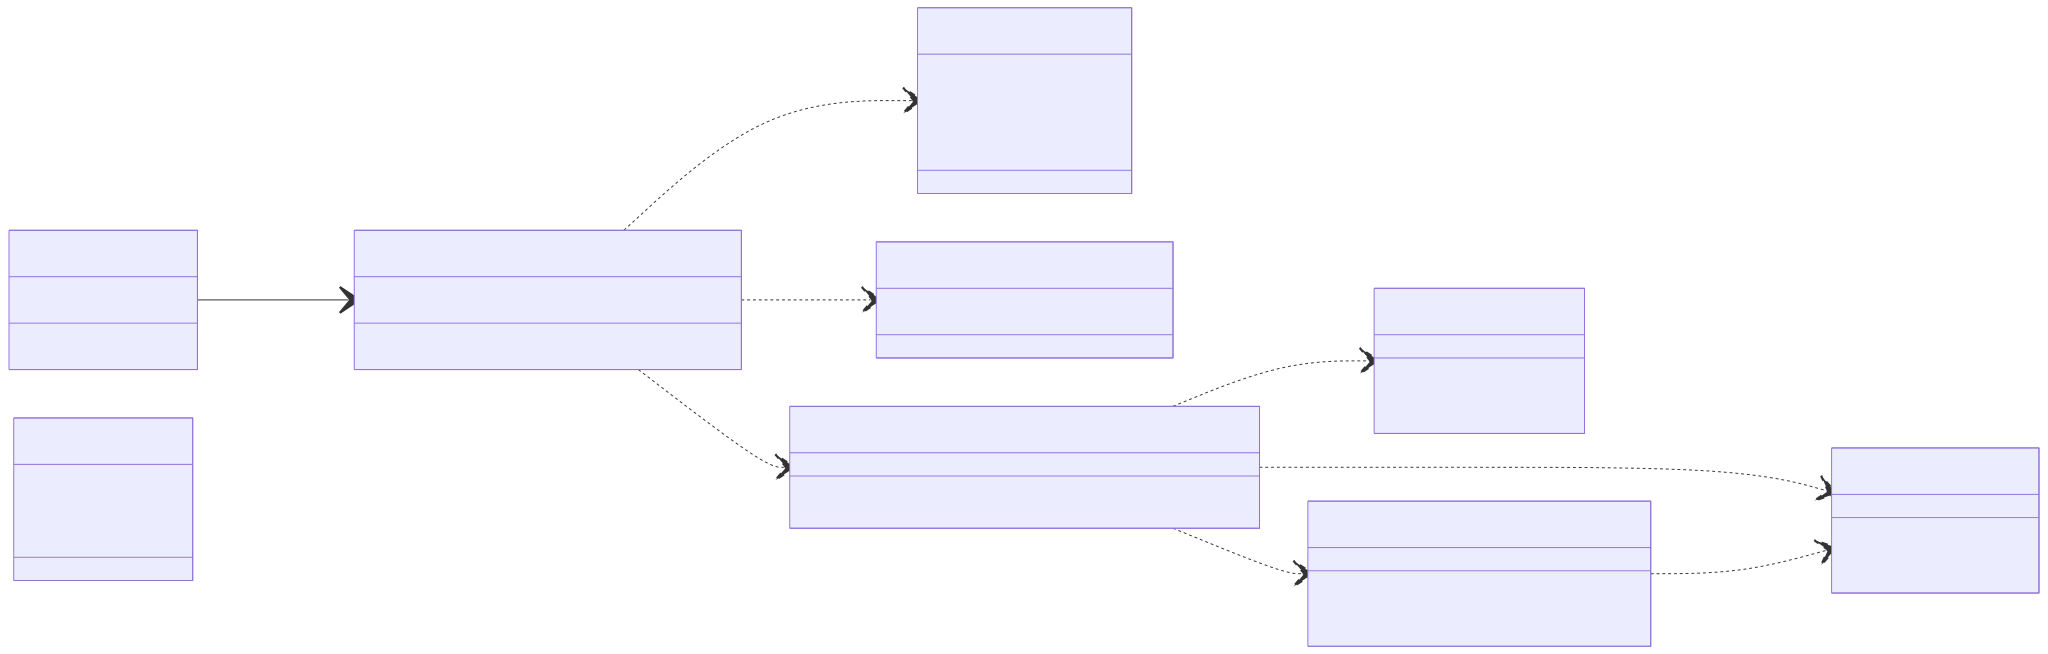
\includegraphics[width=\linewidth]{uml/class-diagram-ai-backend.svg}
  \caption{AI backend architecture.}
\end{figure}

\quad The ai_backend is a FastAPI app that exposes a recommendation endpoint. The entrypoint (Main) creates the FastAPI app, adds CORS middleware, and includes the RecommendationRouter. The router defines the recommend(...) endpoint, which accepts a RecommendationRequest (user_id, query, top_k, filters) and returns a RecommendationResponse containing a list of ItemScore (place_id, score, explanation).

\newpage

\begin{figure}[h]
  \centering
  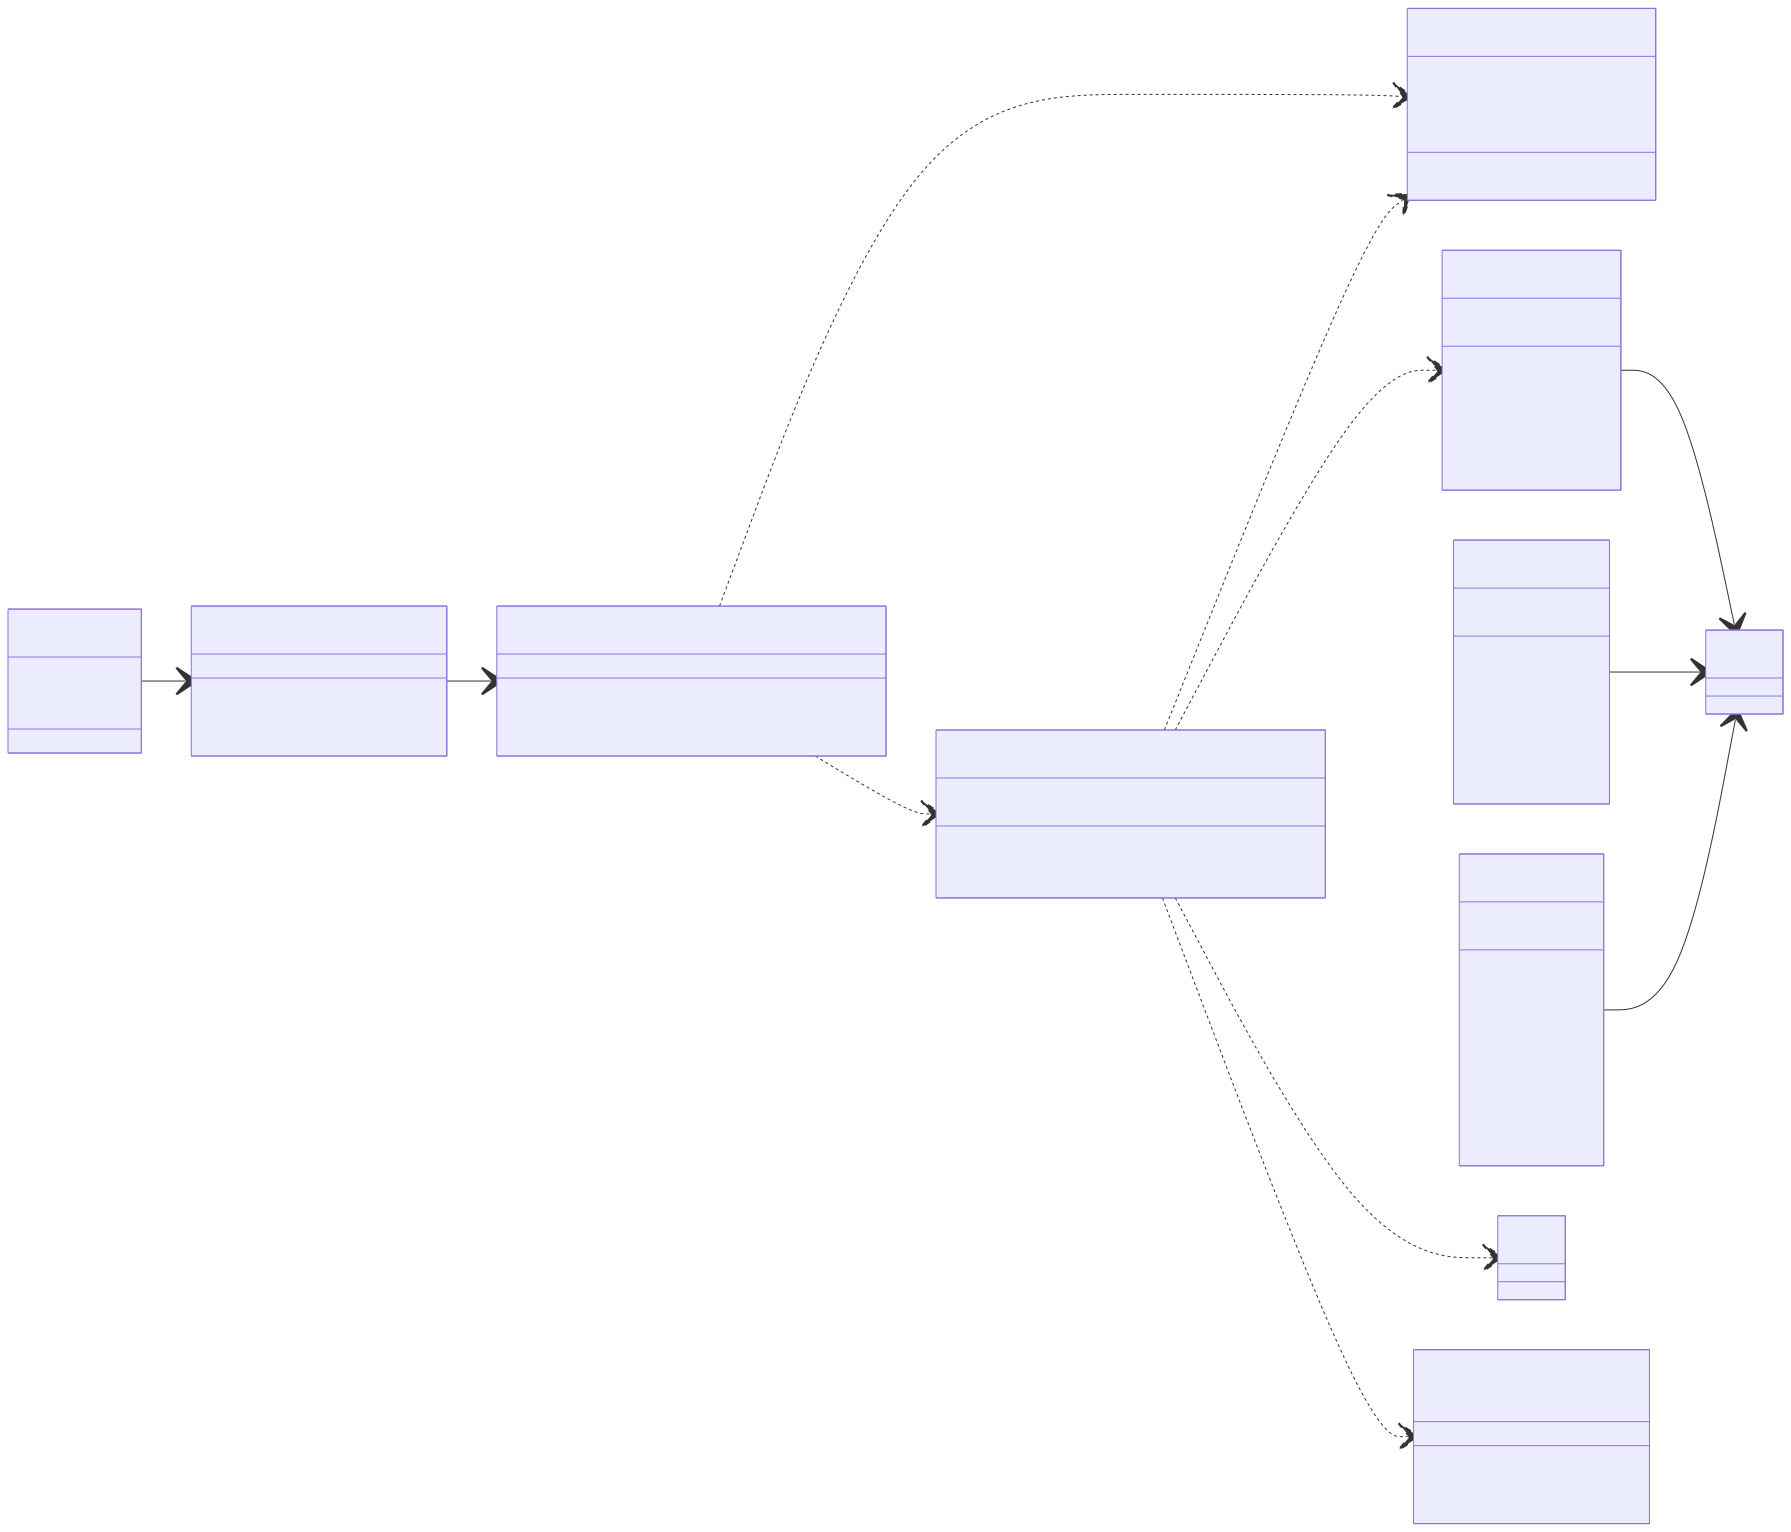
\includegraphics[width=\linewidth]{uml/class-diagram-backend.svg}
  \caption{Backend architecture.}
\end{figure}

\quad The backend is an Express app that wires routes to controllers and services. The entry `App` holds the Express instance and registers `RecommendationRoutes`, which map HTTP handlers to `RecommendationController`. Controllers delegate to `RecommendationService` to call the Python AI backend via Axios and wrap responses in `ServiceResponse`. Enmap-backed stores (`UserDB`, `LocationDB`, `EventDB`) provide simple persistence layers for user state, geocoded locations, and events. `RecommendationService` depends on these stores to enrich requests and cache results, while also calling the external `PythonRecAPI` for recommendations and feedback.

\begin{figure}[h]
  \centering
  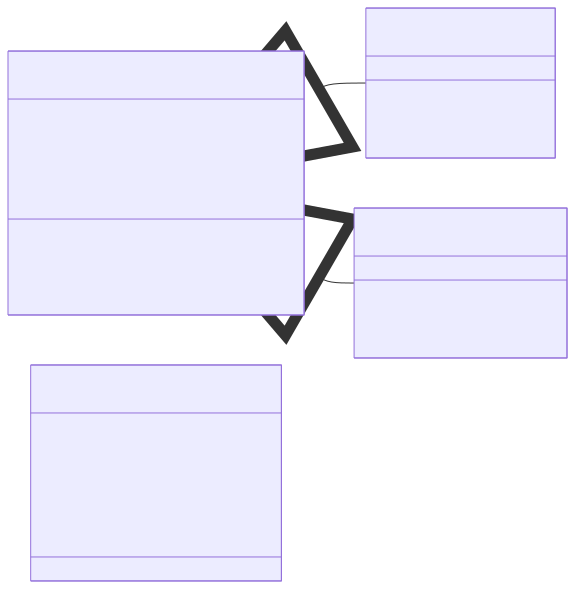
\includegraphics[width=\linewidth]{uml/class-diagram-db.svg}
  \caption{Database architecture.}
\end{figure}

\quad The data layer loads CSVs into DataFrames, builds text+metadata docs, and keeps stable IDs (geo keys or MD5 fallback). BaseColInfo centralizes this; ArchColInfo and RestaurantColInfo tailor narratives for architecture and food. Outputs feed ChromaDB (vector) and BM25 (keyword) search, fused and reranked before the FastAPI /search endpoint returns scored items.

\section{Test Cases and Scenarios}
\lipsum[1-3]
\section{Completed Feature}
Throughout the 10 weeks of development, the application has undergone multiple stages and underhauls. Throughout every development iteration, we aim to pack in as much features as possible. These features include
\begin{itemize}
	\item A functional profiling system, including secure registration and login, user data, and a stable URI that every user has pointing to their user data.
	\item Map display and highlights for locations and routes.
	\item AI-powered tools that fetches a user's possible interested places for recommendation.
	\item Events creation and participation
	\item Geocoding, reverse-geocoding, route finding and nearby location search.
	\item AI-powered location searching to ensure accuracy in semantics and syntax.
\end{itemize}
\section{Planning}
\lipsum[1-2]
\section{Technical Solution and Architecture}
The project, in its core, is a Flutter mobile application that utilizes a NodeJS backend with assistance from Python backend servers that form into a single clean API that the frontend can use. The project's overall architecture can be split into three main architecture styles: the system-level architecture, the client architecture and the backend architecture.

\paragraph{System level architecture.} The interaction between the frontend and the backend is a classic three-tier client-server architecture. More specifically, the Flutter client, which we call the \textit{presentation}, utilizes the Node and Python API (the \textit{application}). The backend then utilizes the database and external services to parse upstream data and pass it to the downstream clients. This is the simplest architecture for an MVP achievable within a reasonable time frame.

\paragraph{Client architecture.} The frontend is primarily developed vertically via a feature-first architecture. The codebase can be grouped by separate features (including but not limited to login, map screen, trips, saved place, location searching), each has its own logic and UI implementation. We choose this architecture because it is a simple and intuitive architecture primarily derived from the user flow. This ensures ease of development and understanding from the team.

\paragraph{Backend architecture.} The backend is a NodeJS express app comprising of multiple endpoints grouped into categories callable from the frontend via dio. In its core, it is an MVC architecture. An endpoint is structured by the core logic's within its service function, express handling and parameters fetching within its controller functions, and routing via an express's Router object. Middlewares for authorization and checking are also included, allowing decoupling and reducing code duplication. Other minor backend servers are also made for training AIs and AI-based searching, and the main backend calls these servers via Cloudflare tunnels. This allows for separation of duties and dependency decoupling.

\begin{figure}[!h]
  \includegraphics[width=\linewidth]{externals/uml/projectModules.png}
\end{figure}
\section{Conclusion and Future Development}


\end{document}